This section evaluates the performance of the cached profile implementation using modern benchmark suites.
\section{Setup}
\label{s:perf_setup}
To provide reliable and comparable results all tests were done on a single node of the Data Center Observatory provided by ETH \cite{ethdco}.
A node features 2 8-Core AMD Opteron 6212 CPUs running at 2600 MHz with 128 GB of DDR3 RAM.
The node is running Fedora 19 and GCC 4.8.3. All JDK builds got created on the node itself.
\\\\
To compare performance the following benchmarks were used:
\begin{enumerate}
  \item \textbf{SPECjvm 2008:} A benchmark suite developed by Standard Performance Evaluation Corporation for measuring the performance of the Java Runtime Environment \cite{specjvm}.  I use version 2008 and I run a subset of 17 out of a total of 21 benchmarks. 4 are omitted due to incompatibility with openJDK 1.9.0.
  \\
  Once finished, SPECjvm prints out the number of operations per minute. This is used to compare the performance and higher is better.
  \item \textbf{Octane 2.0:} A benchmark developed by Google to measure the performance of JavaScript code found in large, real-world applications \cite{octane}. Octane runs on Nashorn, a JavaScript Engine on top of Hotspot. The version used is 2.0 and consists of 17 individual benchmarks of which 16 are used.
  \\
  Octane gives each benchmark a score reflecting the performance, the higher the score, the better the performance.
\end{enumerate}
The benchmarking process was automated using a number of self-written python scripts. The graphs in this chapter always show the arithmetic mean of 50 runs and the error bars display the 95\% confidence intervals.

\section{Startup performance}
\label{s:perf_general}
The main goal of cached profiles is to improve the startup performance of the JVM. Having a rich profile from an earlier execution will allow the JIT compiler to use a highly optimized version right from the beginning.
I will start by looking at SPECjvm since it offers ways to focus on the warmup. An individual description of each benchmark being used can be found in Appendix \ref{a:specjvm_benchmarks}.
\\\\
The longer a program is running the less impact a faster warmup has. Considering most benchmarks include a warmup phase which does not count towards the final score simply running the complete benchmark suite is not an option.
Instead I limited SPECjvm to 1 single operation which, depending on the benchmark take around 10 to 20 seconds.
Additionally, the JVM gets restarted between each single benchmark to prevent methods shared between benchmarks being compiled already.
\\\\
I run each benchmark with all cached profiling features disabled. This run is called the \textit{baseline}     and displays the current openJDK 1.9.0 performance.    
\\\\ 
I then use a single benchmark run where I dump the profiles to disk. This run is not limited to a single operation and instead uses the default values of the benchmark. By default the benchmark is limited by time and runs for about 6 minutes. The idea is that these profiles include information that are usually not available during warmup and result in less deoptimizations and better code quality.
\\\\
These profiles are then used in 3 individual runs using the introduced \texttt{-XX:CacheProfiles} flag. Each run is using one of the 3 different CacheProfilesModes.
\begin{figure}[ht]
  \begin{center}
    \centering
    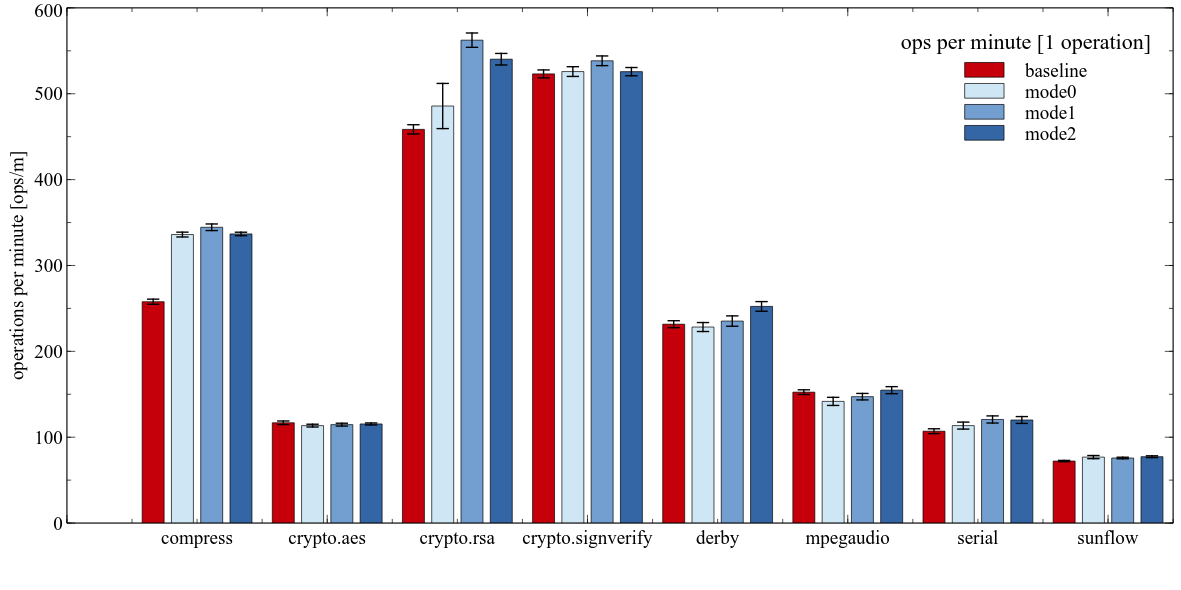
\includegraphics[width=1.0\textwidth]{figures/others_warmup.png}
    \caption{SPECjvm benchmarks on all different modes}
    \label{f:others_warmup}
  \end{center}
\end{figure}
Figures \ref{f:others_warmup} and \ref{f:scimark_warmup} shows the number of operations per minute, measured for each benchmark individually.
The 

\begin{figure}[ht]
  \begin{center}
    \centering
    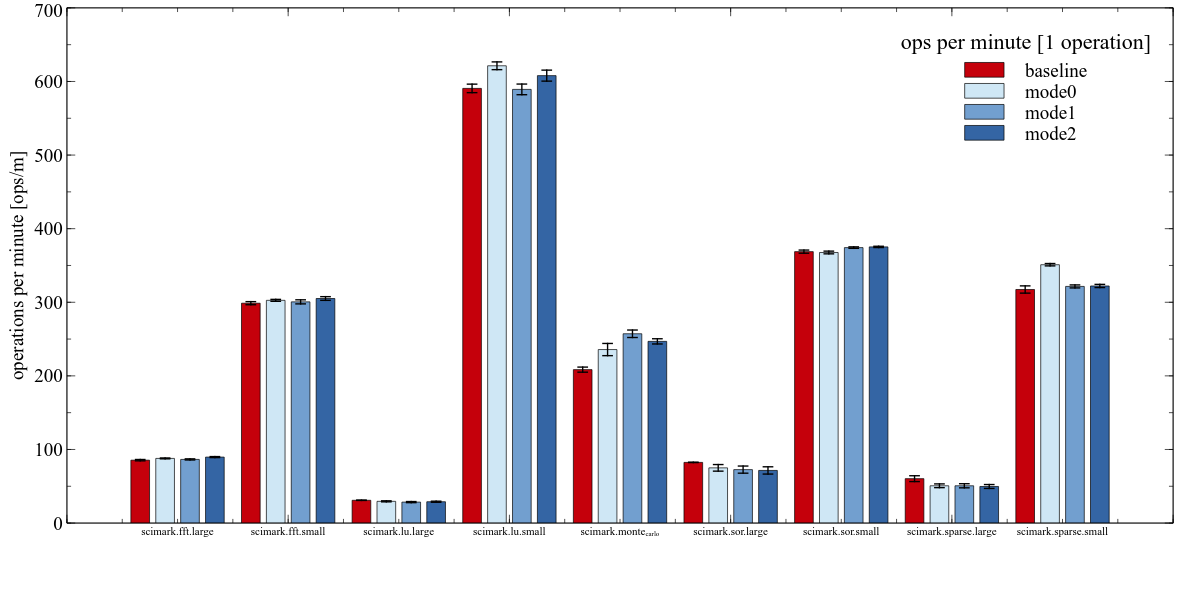
\includegraphics[width=1.0\textwidth]{figures/scimark_warmup.png}
    \caption{SPECjvm scimark benchmarks on all different modes}
    \label{f:scimark_warmup}
  \end{center}
\end{figure}

\begin{figure}[ht]
  \begin{center}
    \centering
    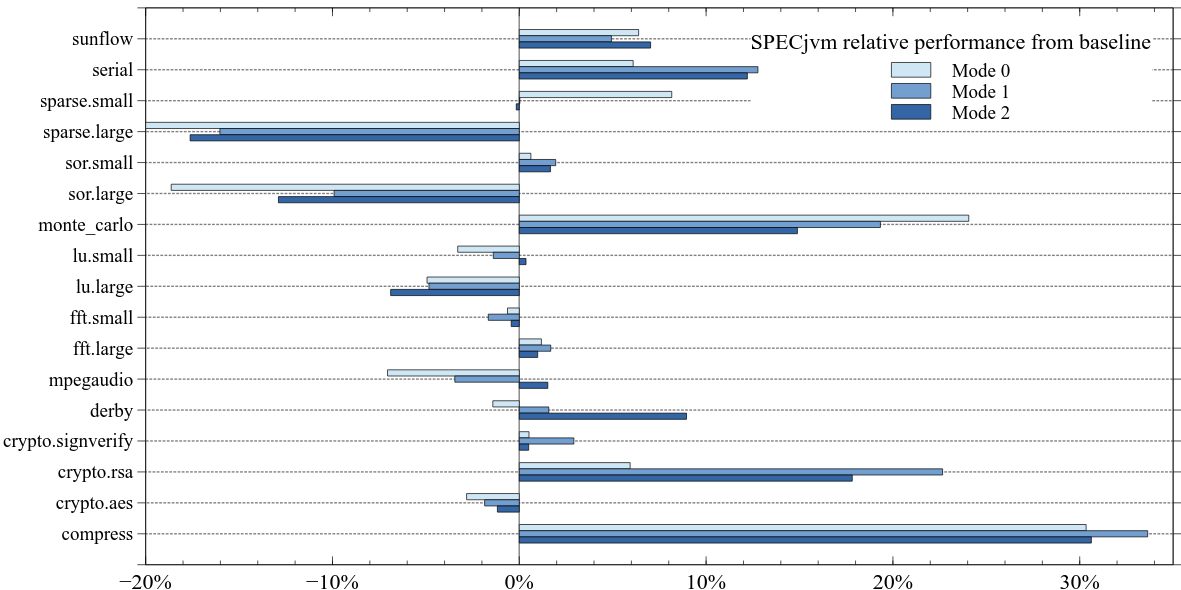
\includegraphics[width=1.0\textwidth]{figures/all_warmup_variation.png}
    \caption{}
    \label{f:all_warmup_variation}
  \end{center}
\end{figure}



\begin{figure}[ht]
  \begin{center}
    \centering
    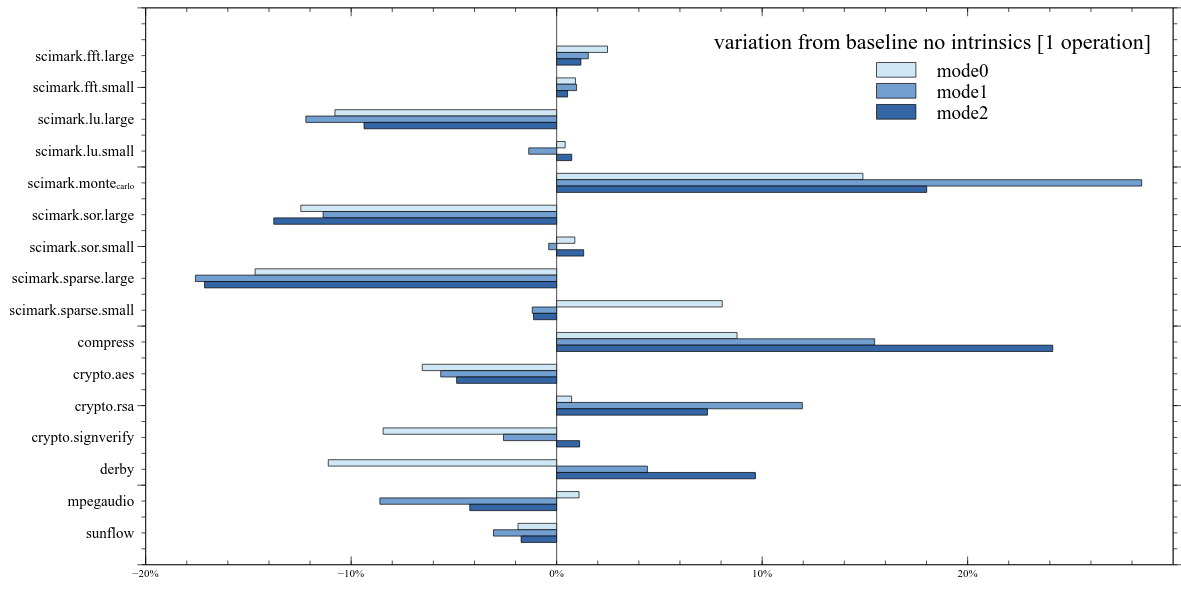
\includegraphics[width=1.0\textwidth]{figures/all_warmup_nointrinsics_variation.png}
    \caption{}
    \label{f:all_warmup_nointrinsics_variation}
  \end{center}
\end{figure}

\section{Deoptimizations}
\label{s:perf_deoptimizations}

\begin{figure}[ht]
  \begin{center}
    \centering
    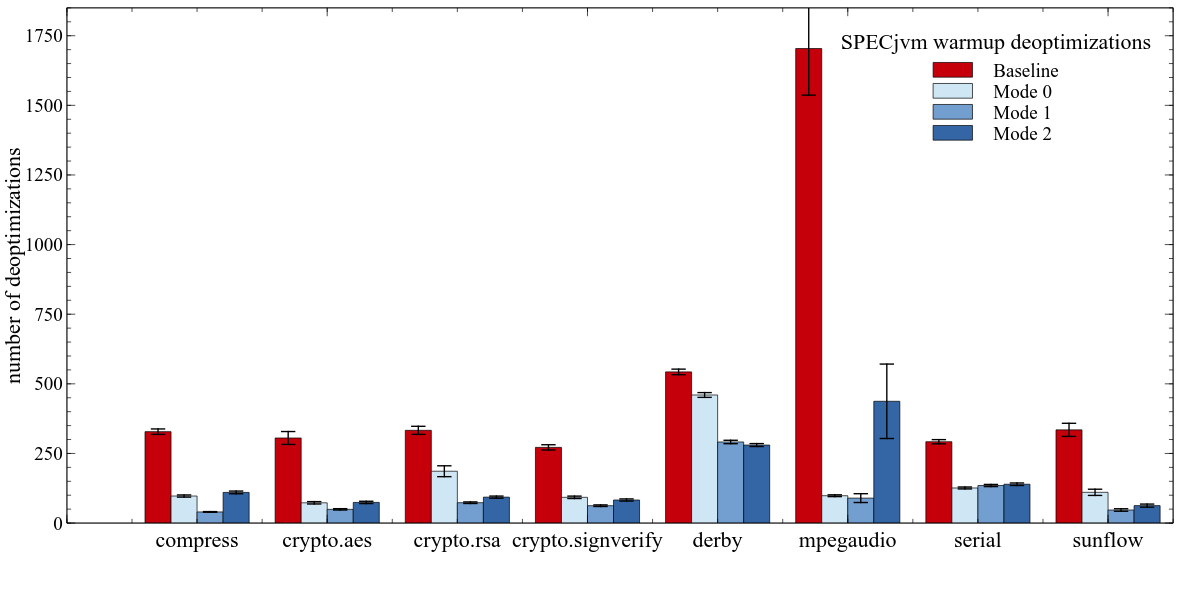
\includegraphics[width=1.0\textwidth]{figures/others_warmup_deopt.png}
    \caption{}
    \label{f:others_warmup_deopt}
  \end{center}
\end{figure}

\begin{figure}[ht]
  \begin{center}
    \centering
    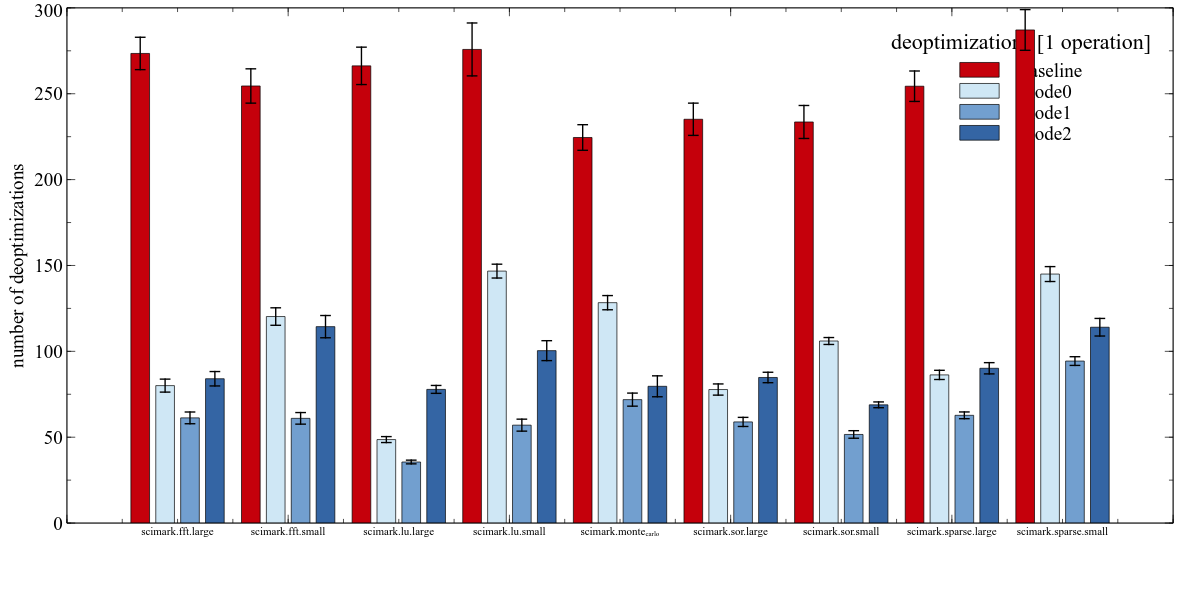
\includegraphics[width=1.0\textwidth]{figures/scimark_warmup_deopt.png}
    \caption{}
    \label{f:scimark_warmup_deopt}
  \end{center}
\end{figure}



\section{Effect on compile queue}
\label{s:perf_compilequeue}
